\documentclass{article} %A4
\usepackage[a4paper,left=1.9cm, right=2.1cm,top = 1.2cm,bottom=2.3cm]{geometry}
\usepackage[utf8]{inputenc}%Umlaute
\usepackage[ngerman]{babel} %Texttrennung
\usepackage{graphicx}	%Grafiken
\usepackage{amssymb}
\usepackage{amsmath}
\usepackage{amsthm}
\usepackage{url}
\usepackage{listings}
 \usepackage{color}
\usepackage{hyperref}
\usepackage{framed}
\usepackage{algpseudocode}
\usepackage{tikz}
\usepackage{sgame}
\usepackage[labelformat=empty]{caption}

\title{Zusammenfassung - Multi-Agenten-Systeme}
\author{
	Andreas Ruscheinski,
}
\begin{document}
\maketitle
\begin{framed}Korrektheit und Vollständigkeit der Informationen sind nicht gewährleistet.
Macht euch eigene Notizen oder ergänzt/korrigiert meine Ausführungen!
\end{framed}
\setcounter{tocdepth}{1}
\tableofcontents

\section{Einführung}
	\subsection{Definition}
	\begin{itemize}
		\item Ein Agent ist ein Computer System welches \textbf{selbstständig} Aktionen im Interesse des Benutzers ausführen kann.
		\item Ein Agent \textbf{befindet} sich in einer \textbf{dynamischen Umgebung} befindet mit welcher er interagiert.
		\item Ein Multi-Agenten-System besteht aus \textbf{mehreren Agenten}, welchee \textbf{miteinander agieren}.
		\item In einem Multi-Agenten-System ist es notwendig für \textbf{erfolgreiche Interaktion} dass Agenten miteinander \textbf{kooperieren},\textbf{ sich abstimmen} und miteinander \textbf{verhandeln} können.
	\end{itemize}
	\subsection{Eigenschaften}
	\begin{itemize}
		\item Jeder Agent hat \textbf{keine vollständigen Informationen} über die Umgebung
		\item Es gibt \textbf{keine globale Kontrolle} der Agenten
		\item Die Daten sind \textbf{dezentralisiert}
		\item Die Berechnung erfolgt \textbf{asynchron}
	\end{itemize}
	\subsection{Gründe für den Einsatz von MAS}
	\begin{itemize}
		\item Problem kann nicht zentralisiert gelöst werden da die \textbf{Ressourcen limitiert} sind
		\item \textbf{Reduktion der Ausfall-Wahrscheinlichkeit} in gegenüber einem zentralisierten System
		\item \textbf{Gewährleistung der inter-konnektion und inter-operation} von verschiedenen Systemen
		\item Lösung von Problemen welche eine\textbf{ Menge aus autonomen Komponenten behandeln}
	\end{itemize}
	\subsection{Konkrete Anwendungsgebiete}
	\begin{itemize}
		\item Clound-Management
		\item Ubiquitous Computing
		\item Grid-Software
		\item Spiele
		\item Verschiedene Gebiete der Industrie (Car-Assembly, Factory Management)
		\item Simulation
	\end{itemize}
	
\section{Rolle der Logik in MAS}
	\subsection{Gründe für Logik}
	\begin{itemize}
		\item Wissensbasis + Aktionen mit Voraussetzung und Auswirkung $\rightarrow$ Plan für Lösung des Problems
		\item Verwaltung von Annahmen
		\item Logik ist ein Framework für das Verstehen von Systemen
		\item Verifikation, Ausführungsspezifikation, Planung
		\item Agenten als Theorembeweiser
	\end{itemize}
	\subsection{Logik-basierende Architektur}
	\begin{itemize}
		\item Grundidee: Beschreibung einer Regelmenge für die Beschreibung der besten Aktion für einen gegeben Zustand
		\item Bestandteile:
		\begin{itemize}
			\item $p$: eine Theorie (eine Menge von Regeln)
			\item $\Delta$: Datenbank mit den aktuellen Zustand der Welt
			\item $A$: eine Menge von Aktionen welcher ein Agent ausführen kann
			\item $\Delta\vdash_{p}\phi$: d.h. $\phi$ kann aus der $\Delta$ unter der Verwendung von $p$ abgeleitet werden, mit $\phi=$Do(a) können wir aus den aktuellen Zustand der Welt auf die bestmögliche Aktion logisch schließen
		\end{itemize}
		 \item Algorithmus-Bestandteile (unabhängig von verwendeter Logik)
		 \begin{itemize}
		 	\item see(s,p), generiert Beobachtung aus der neuen Welt (schwer siehe Vorlesung Mustererkennung und Kontextanalyse)
		 	\item next($\Delta$,p), update der Datenbank mit der Beobachtung
		 	\item action($\Delta$), ermittelt die auszuführende Aktion aus der Datenbank, entweder ist die Aktion direkt beschrieben oder kann aus den Regeln abgeleitet werden kann
		 \end{itemize}
		 \item Algorithmus - Ermittelung einer Aktion aus einer Wissensdatenbank:
		 \begin{enumerate}
		 	\item Überprüfe für jede Aktion a ob  $\Delta\vdash_{p}Do(a)$ gilt (d.h. a kann direkt abgeleitet werden)
		 	\item Falls ja: gebe a zurück sonst
		 	\item Überprüfe für jede Aktion a ob $\Delta\not{\vdash}_{p}\neg Do(a)$ gilt (d.h a ist nicht explizit ausgeschlossen)
		 	\item Falls ja: gebe a zurück sonst gebe NULL zurück (keine Aktion gefunden)
		 \end{enumerate}
	\end{itemize}
	\subsection{Modal Logik}
	\begin{itemize}
		\item Erlaubt Ausdrücke wie: wahrscheinlich wahr, geglaubt wahr, wahr in der Zukunft usw.
		\item kann genutzt werden um Informationen für die Agenten abzuleiten und über das Wissen von Agenten zu schließen
		\item Syntax:
		\begin{itemize}
			\item Prädikatenlogik mit Erweiterung
			\item Prop: eine Menge von atomaren Formeln
			\item wenn $p,q \in Prob$ dann sind auch $\neg p, p \& q, \diamond p,\square p$ Formeln
			\item $\diamond$ p: möglicherweise p, manchmal p 
			\item $\square$p: immer p, notwendigerweise p
		\end{itemize}
		\item Semantik:
		\begin{itemize}
			\item Kripke-Struktur: $<W,R,\mu>$
			\begin{description}
				\item[$W$] eine Menge von Welten
				\item[$R$] eine Menge von binär Relationen, beschreiben den Übergang zwischen den Welten
				\item[$\mu$] Abbildungsfunktion welche jeder Welt Eigenschaften zuordnet ($\mu : W \rightarrow 2^{Prop}$)
			\end{description}
			\item Definition von $\diamond$ und $\square$ Operator auf Basis von Erreichbarkeit der Welten in einer Kripke-Struktur
			\item $\square p$: p ist wahr in allen Welten, welche von der aktuellen Welt erreichbar sind
			\item $<M,w>\vDash\square p$ wenn für alle $w' \in W$ gilt: wenn $(w,w') \in R$ denn $<M,w'>\vDash p$
			\item $\diamond p$: p ist wahr, wenn mindestens eine Welt erreichbar in welcher p wahr ist
			\item $<M,w>\vDash\diamond p$ wenn es ein $w' \in W$ existiert mit:  wenn $(w,w') \in R$ denn $<M,w'>\vDash p$
			\item für R muss zusätzlich gelten:
			\begin{description}
				\item[reflexiv] für jedes $x \in W$ gilt $R(x,x)$ d.h. x ist von x aus erreichbar
				\item[transitiv] für jedes $x,y,z \in W$ gilt $R(x,y) \wedge R(y,z) \implies R(x,z)$ d.h. wenn man von x nach y und von y nach z gehen kann, kann man auch von x nach z gehen
				\item[seriell] für jedes $x \in W$ existiert ein $y$ so dass gilt $R(x,y)$ d.h. für jede Welt ist mit einer anderen Welt in Relation
				\item[euklidisch] wenn für jedes $x,y,z \in W$ mit $R(x,y)$ und $R(x,z)$ gilt auch $R(y,z)$ d.h. wenn man von x nach y und von x nach z gehen kann dann kann man auch von y nach z gehen 
			\end{description}
			\item Axiome (Beschreiben Eigenschaften für $R$):
			\begin{description}
				\item[$\square p \Rightarrow p$] Wenn immer $p$ gilt folgt daraus das aktuell p gilt (Reflexiv)
				\item[$\square p \Rightarrow \diamond p$] Wenn $p$ immer wahr ist, ist p auch in mindestens einer Welt wahr (Seriell)
				\item[$\square p \Rightarrow \square \square p$] Wenn $p$ ist immer wahr, ist p auch immer wahr wenn wir einen Übergang machen (transitiv)
				\item[$\diamond p \Rightarrow \square \diamond p$] Wenn $p$ in mindestens einer Welt wahr ist, ist p für immer Wahr wenn wir diese Welt erreicht haben (Euklidisch)
			\end{description}
			\item Anwendung der modal Logik auf Agenten durch Einführung von Indizes, welche entsprechend für Agent gelten
			\item Operator - Knowledge: $K_ip$ bedeutet dass Agent i weiss $p$
			\item der Modale Operator $\square_i$ wird zu $K_i$
			\item Axiome und Agenten:
			\begin{description}
				\item[$K_{i}p \Rightarrow p$] Wenn Agent glaubt das p wahr ist, p ist auch in Wirklichkeit wahr
				\item[$K_{i}p \Rightarrow \neg K_{i}\neg p$] Wenn der Agent p glaubt, glaub er nicht die Negation
				\item[$K_{i}p \Rightarrow K_{i}K_{i}^p$] Wenn der Agent p glaubt, weiß er selbst dass er p glaubt
				\item[$\neg K_{i}\neg p \Rightarrow K_{i}\neg K_{i}\neg p$] Wenn der Agent nicht p glaubt, weiß er dass er nicht p glaubt.
			\end{description}
			\item es gilt: $<M,w> \vDash K_i p$ genau dann wenn $\forall w' \in W$ gilt: wenn $(w,w') \in R_i$ denn $<M,w'> \vDash p$ (vgl. Definition von $\square$)
			\item Probleme:
			\begin{itemize}
				\item Agent glaubt alles was wahr ist incl. Tautologien: wenn $\vDash p$ denn $K_i p$
				\item Agent weiss alle Schlussfolgerungen des eigenen Wissens: $\vDash p \rightarrow q$ denn $\vDash K_i p \rightarrow K_i q$ (Kripke Axiom: $K_i(p\rightarrow q) \rightarrow (K_i p \rightarrow K_i q)$)
				\item Menschliches wissen ist oft inkonsistent
				\item Menschen glauben nicht alle equivalenten Aussagen
			\end{itemize}
		\end{itemize}
	\end{itemize}
	\subsection{BDI-Logic}
	\begin{itemize}
		\item Klassisch logischer Operatoren: und, oder, negation usw...
		\item CTL* Path Quantifikatoren
		\begin{itemize}
			\item $A \phi$: es gilt auf allen Pfaden $\phi$
			\item $E \phi$: es gilt auf einigen Pfaden $\phi$
			\item $G$: global
			\item $F$: zukünftig
		\end{itemize}
		\item BDI-Funktionen:
		\begin{itemize}
			\item (Bel i $\phi$): i glaubt $\phi$
			\item (Des i $\phi$): i will $\phi$
			\item (Int i $\phi$): i verfolgt $\phi$
		\end{itemize}
		\item Regeln:
		\begin{itemize}
			\item (Des $\alpha$) $\rightarrow$ (Bel $\alpha$) (Belief goal compatibility): Wenn der Agent $\alpha$ erreichen will folgt daraus das der Agent $\alpha$ glaubt
			\item (Int $\alpha$) $\rightarrow$ (Des $\alpha$) (Goal-intention compatibility): Wenn der Agent $\alpha$ verfolgt daraus das der Agent $\alpha$ erreichen will
			\item (Int does(a)) $\rightarrow$ does(a) (Volitional commitment): Wenn der Agent does(a) ausführen möchte, wird er diese als nächstes ausführen
			\item (Des $\alpha$) $\rightarrow$ (Bel (Des $\alpha$)) und (Int $\alpha$) $\rightarrow$ (Bel (Int $\alpha$)) (Awareness of goals \& intentions): Bedingt dass neue Ziele und Intentionen als Event gepostet werden müssen in der Wissensbasis
			\item done(a) $\rightarrow$ (Bel (done(a))) (No unconscious actions): Wenn ein Agent eine Aktion ausgeführt hat weiss er das er diese ausgeführt hat
			\item (Int $\alpha$) $\rightarrow$ AF($\neg$(Int $\alpha$)) (No infinite deferral): Ein Agent will eventuell eine Intention verfolgen oder diese Verwerfen
		\end{itemize}
		\item reactive und proactive Agenten
		\begin{itemize}
			\item reactiv: Aktion wird ausgeführt durch eine Eingabe: wenn Eingabe = p denn tue a
			\item proactiv: Planung und Ausführung von Aktionen um ein Ziel zu erreichen: tue a um p zu erreichen
		\end{itemize}
	\end{itemize}
	
\section{Planning}
	\subsection{Einführung - Brooks Vision}
	\begin{itemize}
		\item Ziel 1: Intelligentes Verhalten ohne explizite Repräsentation des Wissens
		\item Ziel 2: Intelligenten Verhalten ohne abstraktes schließen über die Repräsentation des Wissens
		\item Idee 1: Echte Intelligenz gibt es nur ein einer Welt und nicht losgelöst von dieser wie in Theorem Beweisern und Expertensysteme
		\item Idee 2: Intelligentes Verhalten entsteht erst als Ergebnis der Interaktion mit der Umgebung
	\end{itemize}
	\subsection{Subsumtion Architektur}
	\begin{itemize}
		\item Traditionell: Die Intelligenz steht zwischen Beobachtung und Aktion d.h. aus Beobachtungen wird geschlossen welche Aktion ausgeführt wird
		\item Neu: Die Intelligenz entsteht beim Beobachter durch die Aktionen in der Welt d.h. ein Agent ist nicht an sich intelligent sondern wirkt intelligent für einen Beobachter
		\item Entscheidungsfindung durch verschiedene Aufgaben:
		\begin{itemize}
			\item Verhalten ist eine Abbildung von Zustand auf Aktion
			\item Verarbeitung der Sensorwerte mit Schluss auf den Zustand
			\item Zustände und Aktionen sind direkt gekoppelt
		\end{itemize}
		\item Mechanismus für die Auswahl der Aktionen: Prioritäten d.h Verhalten mit hoher Priorität kann Verhalten mit niedrigeren Prioritäten unterdrücken
		\item Formales Modell:
		\begin{itemize}
			\item Ein Verhalten (Behavior) $b \in Beh$ ist ein Tupel $(c,a)$ mit $c \subseteq P, a \in A$ wobei P ist eine Menge von Beobachtungen und A eine Menge von Aktionen
			\item Ein Verhalten wird ausgeführt wenn die Umgebung sich in dem Zustand $s\in S$ befindet und $see(s) \in c$
			\item Subsumption Hierachie wird realisiert durch eine Hemmungs-Relation $b_{1} \prec b_{2}$ ($b_{1}$ hemmt $b_{2}$ d.h. $b_{1}$ hat eine höhere Priorität)
		\end{itemize}
		\item Aktionsauswahl-Algorithmus:
		\begin{enumerate}
			\item Berechne die Menge von aktivierbaren Aktionen $FB = \{(c,a)|(c,a)\in Beh \wedge see(s)\in c\}$
			\item für jede Aktion in FB überprüfe ob es eine Aktion in FB gibt welche eine höhere Priorität hat
			\item wenn es keine Aktion mit höherer Priorität gefunden wurde: gib $a$ zurück sonst: NULL (Keine Aktion gefunden)
		\end{enumerate}
		\item Vorteile:
		\begin{itemize}
			\item Einfach und hohe Ausdrucksfähigkeit
			\item Die Berechnung ist einfach nach zu vollziehen
			\item Robust gegen Ausfälle
			\item Das gesamte Verhalten entsteht durch Interaktion mit der Umwelt
		\end{itemize}
		\item Nachteile:
		\begin{itemize}
			\item Verhalten wird hard codiert unter der Annahme die Umgebung genau zu kennen
			\item Schwierige Entscheidung über das Standard Verhalten
			\item langwierige Entscheidungen schwer möglich
			\item skaliert nicht in größeren Systemen
		\end{itemize}
	\end{itemize}
	\subsection{Planung}
	\begin{itemize}
		\item Grundideen:
		\begin{itemize}
			\item Beschreibung des Zieles (Intention) welches erreicht werden soll
			\item Beschreibung der Aktionen welche ausgeführt werden kann
			\item Beschreibung der Umgebung
			\item Beschreibungen + Planner = Plan welches das Ziel erreicht
		\end{itemize}
		\item Umsetzung durch z.B STRIPS Planner
		\begin{itemize}
			\item Repräsentation der Umgebung durch Ontologie (Begriffe + Relationen)
			\item Beschreibung der aktuellen Welt durch Verwendung der Ontologie Begriffe (closed world assumption: alles was nicht angegeben wird ist falsch)
			\item Jede Aktion hat Name, Pre-Condition List (alle Bedingungen müssen wahr sein bevor Aktion ausgeführt werden kann), Delete-List (Bedingungen welche nach der Ausführung nicht mehr wahr sind), Add-List (Bedingungen welche nach der Ausführung der Aktion gelten) (können alle Variablen erhalten für allgemeine Aussagen)
		\end{itemize}
		\item Ein Plan ist eine Liste von Aktionen, mit Variablen ersetzt durch Konstanten. Die Ausführung der Aktionen führt von den aktuellen Zustand in ein einen Zustand, welcher das Ziel erfüllt. Der Plan ist vollständig (keine weiteren Aktionen notwendig) und konsistent (alle Pre-Conditions sind erfüllt) und die Schritte können hintereinander ausgeführt werden ohne dass die Ausführung eines Schrittes beeinflusst wird.
		\item Formal: partielly ordered Plans
		\begin{itemize}
			\item Plan Schritt mit Partieller Ordnung $\prec$: $S_{i} \prec S_{j}$ bedeutet dass $S_{i}$ vor $S_{j}$ ausgeführt werden muss
			\item Eine Menge von Variablen Zuordnungen $x=t$ mit x ist eine Variable und t ist eine Konstante
			\item Eine Menge von Kausalen Relationen: $S_{i} \rightarrow S_{j}$ bedeutet die Ausführung $S_{i}$ macht die Vorbedingungen von $S_{j}$ wahr (impliziert  $S_{i} \prec S_{j}$)
		\end{itemize}
		\item Formal: Eigenschaften Konsistenz und Vollständigkeit
		\begin{itemize}
			\item Vollständigkeit: 
			\begin{itemize}
				\item es gilt: $\forall S_{j}$ mit $c\in Precond(S_{j})$ und $\exists S_{i}$ mit $S_{i} \prec S_{j}$ und $c\in Effect(S_{i})$ (die Vorbedingungen für $S_{j}$ sind Teil des Effektes von $S_{i}$)
				\item für eine Sequenz gilt:$\forall S_{k}$ mit $S_{i} \prec S_{k} \prec S_{j}, \neg c \notin Effect S_{k}$
			\end{itemize} 
			\item Konsistenz: Wenn $S_{i} \prec S_{j}$ denn $S_{j} \prec S_{i}$ und wenn $x=A$ denn $x \neq B$ für verschiedene A und B für die Variable x.
		\end{itemize}
		\item Vorlesungfolien für Beispiel!!!
		\item iterative Erstellung eines Plans durch rückwärts anwenden der Regeln d.h. in jedem Schritt wird eine offene Bedingung durch die entsprechende Aktion erfüllt
		\item dadurch können Konflikte entstehen
		\begin{itemize}
			\item Ein Konflikt gdw. wenn $S_{3}$ bedroht die kausale Ordnung zwischen $S_{1}$ und $S_{2}$
			\item Lösung 1: Demotion - $S_{3}$ vor $S_{1}$ und $S_{2}$ ausführen
			\item Lösung 2: Promotion - $S_{3}$ nach $S_{1}$ und $S_{2}$ ausführen
			\item sollte dies wieder zu Konflikte führen Backtrack und eine andere Lösung ausprobieren in dem $S_{3}$ neben $S_{1}$ zu $S_{2}$ eingeordnet wird
		\end{itemize}
	\end{itemize}
	\subsection{Planning Agents}
	\begin{itemize}
		\item Erster Ansatz für den Planning Agent:
		\begin{enumerate}
			\item beobachte die Umgebung
			\item aktualisiere das interne Modell der Umgebung
			\item ermittle welche Intention als nächstes erreicht werden soll
			\item benutze means-end Resoning für die Erstellung des Plans welche die Intention erreicht
			\item führe Plan aus
		\end{enumerate}
		\item means-end Resoning: Gib den Agent eine Repräsentation der Ziele/Intentionen welche erreicht werden sollen, Aktionen welche er ausführen kann, der Umgebung $\rightarrow$ Agent nutzt Repräsentationen um einen Plan zu generieren
		\item Problem: Planung und Ermittelung welches Ziel als nächstes erreicht werden soll kosten Zeit
		\item dadurch kann die Situation entstehen dass der Agent ein Ziel erreichen will welches nach dessen Ermittelung nicht mehr optimal ist
		\item Unter folgenden Annahmen ist die getroffene Entscheidung noch immer optimal: wenn Planung und  Ermittelung schnell genug sind; die Welt sich nicht verändert hat; getroffene Zielentscheidung ist noch immer optimal wenn Agenten Plan gefunden hat;
		\item Agenten Algorithmus formal 1:
		\begin{enumerate}
			\item B = $B_{0}$ - Ausgangs-Beliefs
			\item führe unendlich lange aus:
			\item beobachte Umwelt - p
			\item B = brf(B,p) - Aktualisierung des der eigenen Beliefs
			\item I = deliberate(B) - Ermittelung
			\item $\pi$ = plan(B,I) - Plane
			\item execute($\pi$) - führe Plan aus
		\end{enumerate}
		\item Ermittelung durch: option-generation (Erstelle mögliche Ziele) und filter (Auswahl des Ziels)
		\item option-generation: Nutzt aktuelle Beliefs und Intententions und ermittelt daraus eine Menge von Optionen (Desires)
		\item filter: Der Agent wählt zwischen verschiedenen Alternativen aus den Optionen und beginnt die gewählte Option zu verfolgen	
		\item Agenten Algorithmus formal 2 - BDI Agent:
		\begin{enumerate}
			\item B = $B_{0}$ - Ausgangs-Beliefs
			\item führe unendlich lange aus:
			\item beobachte Umwelt - p
			\item B = brf(B,p) - Aktualisierung des der eigenen Beliefs
			\item D = options(B,i) - Desires (Ziele)
			\item I = filter(B,D,I) - Ermittelung der Intentionen durch Beliefs(Wissen über Umwelt), Desires(Ziele) und Intentions(gewählten Ziel)
			\item $\pi$ = plan(B,I) - Plane
			\item execute($\pi$) - führe Plan aus
		\end{enumerate}
		\item Begriffserklärungen:
		\begin{itemize}
			\item Beliefs - Weltwisssen (Alles was wir wissen d.h. was wir glauben über die Welt, unseren Fähigkeiten und Zielen)
			\item Desires - Ziele (Optionen welche wir gerne erfüllt hätten)
			\item Intentions - Absicht (Ziel welches ich jetzt erreichen möchte)
		\end{itemize}
	\end{itemize}
	\subsection{Commitments}
	\begin{itemize}
		\item Strategien:
		\begin{itemize}
			\item Blind Commitment - Agent will Intention erreichen bis er glaubt die Intention erreicht zu haben
			\item Single-minded Commitment - Agent will Intention erreichen bis er glaubt diese erreicht zu haben oder es nicht mehr möglich ist
			\item Open-minded Commitment - Agent will Intention solange er glaubt dieser erreichen zu können
		\end{itemize}
		\item Anpassungen des Agenten Algorithmus
		\begin{enumerate}
			\item wie bisher $\rightarrow$ Blind Commitment
			\item wie bisher - Ermittle Plan und solange dieser nicht leer ist führe diesen Schrittweise aus, nach jedem Schritt hole neuen Percept + Belief Update: wenn Ziel nicht mehr erreicht werden kann ermittle neuen Plan $\rightarrow$ Single-minded da keine neuen Intentionen erwogen werden
			\item wie bisher - Ermittle Plan und solange dieser nicht leer ist führe diesen Schrittweise aus solange Intention nicht erreicht und dieser noch nicht unmöglich ist, nach jedem Schritt hole neuen Percept + Belief Update + Desires ermitteln + Intentions ermitteln :wenn Ziel nicht mehr erreicht werden kann ermittle neuen Plan
		\end{enumerate}
		\item Problem: Agent will Intentions verfolgen selbst wenn schon klar ist das Ziel nicht mehr erreicht werden kann und Agent will konstant berücksichtigten dass evtl unnötige Zeit verschwendet wurde und deshalb nie dass Ziel erreichen
		\item Lösung: Meta-Level Control welches entscheidet wann der Agent seine Intention verwirft
	\end{itemize}
\section{Kooperation von Agenten}
	\subsection{Einführung}
	\begin{itemize}
		\item Ein Multiagenten System besteht aus mehren Agenten welche
		\begin{itemize}
			\item Interagieren durch Kommunikation
			\item Mit der Umgebung interagieren können
			\item Haben unterschiedliche Einflussbereiche auf die Umgebung
			\item stehen in Beziehungen zu einander (Organisation)
		\end{itemize}
		\item Egoistische Agenten bergen Potential für Konflikte da jeder seine Ziele verfolgen möchte
		\item Lösung: Kooperation mittels Entscheidungstheorie
	\end{itemize}
	\subsection{Entscheidungstheorie - Spieltheorie}
	\begin{itemize}
		\item Wir haben zwei Agenten $A_{i}$ und $A_{j}$
		\item jeder Agent hat die gleiche Menge $\Omega = \{\omega_{1},\omega_{2},\dots\}$ eine Menge von Ergebnissen welche für den Agenten von Bedeutung ist
		\item die Bedeutung für einen Agent i wird durch eine Utilty-Funktion repräsentiert $u_i: \Omega \rightarrow \mathbb{R}$ (jeder Agent hat eine Utility-Funktion)
		\item Utility-Funktion bildet Ordnung der Ergebnisse: $\omega \geq_{i} \omega^{'}$ bedeutet also $u_{i}(\omega) \geq u_{i}(\omega^{'})$
		\item Utility beschreibt den Nutzen nicht GELD!
		\item Modell für mehrere Agenten:
		\begin{itemize}
			\item Agenten wählen Aktion gleichzeitig aus, als Ergebnis etwas aus $\Omega$
			\item das aktuelle Ergebnis hängt von Kombinationen von Aktionen ab
			\item Jeder Agent hat nur zwei mögliche Aktionen: C und D
			\item $\tau: A_{c} \times A_{c} \rightarrow \Omega $ eine Funktion welche die Aktion von den beiden Agenten auf ein Ergebnis abbildet
			\item Eine Welt lässt sich mittels $\tau$ beschreiben unter Verwendung aller möglichen Kombinationen von Aktionen $\rightarrow$ hat ein Ergebnis
			\item jeder Agent kann die Utility von dem Ergebnis berechnen
		\end{itemize}
		\item Darstellung mittels Payoff Matrix (Ein Agent ist Spalte (linker Rechter), ein Agent ist Zeile (linker Eintrag)
		\newline
		\begin{game}{2}{2}
			   & D & C \\
			 D & 1,1 & 1,4\\
			 C & 4,1 & 4,4
		\end{game}
		\item Beispiel: $\tau(D,C) = \omega_{1}$ mit $u_{i}(\omega_{1}) = 1$ und $u_{j}(\omega_{1})=4$
	\end{itemize}
	\subsection{Strategien}
	\begin{itemize}
		\item Dominate-Strategie
		\begin{itemize}
			\item Aus einer gegebenen Strategie s (Beispiel: D oder C) für Agent $i$ ergeben sich verschiedene Ergebnisse ($\omega$)
			\item Strategie $s_{1}$ dominiert Strategie $s_{2}$ wenn jedes Ergebnis wenn $s_{1}$ gespielt wird bevorzugt wird gegenüber $s_{2}$
			\item Rationale Agenten werden niemals dominierte Strategien spielen d.h. es gibt eine Strategie welche besser ist
			\item Ziel: dominierte Strategie eliminieren
			\item Anmerkung: es ist nicht immer möglich nur eine nicht dominierte Strategie zu finden
		\end{itemize}
		\item Nash-Equilibrium (Nash-Gleichgewicht):
		\begin{itemize}
			\item Strategie $s_i$ und $s_j$ sind ein einem Nash-Gleichgewicht gdw: Unter der Annahme dass Agent i spielt $s_i$ und Agent j kann nicht besser sein als wenn er $s_j$ spielt UND unter der Annahme dass Agent j spielt $s_j$ und Agent i kann nicht besser sein als wenn er $s_i$ spielt
			\item Aber: nicht jede Interaktion hat ein Nash-Gleichgewicht und einige Interaktionen haben mehrere Nash-Gleichgewichte
		\end{itemize}
		\item Pareto Optimum:
		\begin{itemize}
			\item Gegeben einer initialen Zuordnung von Gütern für eine Menge von Agenten
			\item Eine Änderung welche für einen Agent besser ist aber für keinen anderen Agenten schlechter nennt sich Pareto-Verbesserung
			\item Eine Zuweisung ist Pareto-Optimal gdw. keine weiteren Pareto-Verbesserungen gemacht werden können
		\end{itemize}
		\item Kompetitive- und Null-Summen-Interaktionen
		\begin{itemize}
			\item Szenarios in denen Agenten gegenläufige Präferenzen haben sind streng kompetitiv
			\item Null-Summen Spiele gdw. die Summe aller Utilitys der Agenten = 0 sind: $u_i(\omega) + u_j(\omega) = 0, \forall \omega \in \Omega$
			\item Null-Summen Spiele sind streng kompetitiv, im Real-Life selten
		\end{itemize}
		\item Beispiel: Prison Dilemma
		\begin{itemize}
			\item zwei Männer wurden verhaftet wegen Diebstahl
			\item wenn jmd gesteht und der andere nicht geht der Geständige 3 Jahre ins Gefängnis und der andere kommt frei
			\item wenn beide gestehen beide gehen für 3 Jahre ins Gefängnis
			\item Wenn keiner gesteht geht jeder 1 Jahr ins Gefängnis
			\item Nash-Equilibirum gdw. jeder gesteht
			\item Besser wäre aber wenn jeder schweigt
		\end{itemize}
		\item Grundlegendes Problem von Multi-Agenten Interaktionen: es wird keine Kooperation entstehen wenn jeder Agent egoistisch ist
		\item Lösung: Annahme mein Gegenspieler ist meine Zwilling, oder Shadow of the Future (nochmaliges treffen in der Zukunft)
		\item Iterated Prison Dilemma
		\begin{itemize}
			\item Lösung: Spiele das Spiel mehrmals
			\item Rückwärts Indutkion: Annahme wir spielen n mal, in Runde n-1 wollen wir schweigen für höheren Payoff, dadurch wird n-2 zur letzten richtigen Runde wo wir auch schweigen würden für höheren Payoff $\dots$ Prison-Dilemma mit fixer Anzahl an Runden ist schweigen immer die beste Strategie
			\item Untersuchung in Axelrods Tournament: Iterated Prison Dilemma gegen verschiedene Gegner
			\item Verschiedene Stragiegien: ALLD (always defect), TIT-FOR-TAT (Kooperation in der ersten Runde, danach immer die Aktion welche der Gegner gespielt hat), TESTER, JOSS
		\end{itemize}
	\end{itemize}
	\subsection{Benevolent Agents}
	\begin{itemize}
		\item Wenn wir das ganze System kontrollieren können wir Agenten bauen welche sich gegenseitig unterstützen
		\item Es gibt Konventionen über das Verhalten
		\item Unter dieser Annahme: Unsere Agenten sind mehr oder weniger gutmütig d.h. unser bestes Ziel ist deren bestes Ziel
		\item gutmütige Agenten vereinfachen das System-Design
		\item gutmütige Agenten haben eigene Interesse kollidieren aber nicht mit anderen Interessen
	\end{itemize}
\section{Agenten Kommunikation}
	\subsection{Einführung}
	\begin{itemize}
		\item Kommunikation ist der Austausch zwischen Informationen
		\item für Kooperation ist es notwendig zu kommunizieren: Speech Acts, KQML \& KIF, FIPA ACL
	\end{itemize}
	\subsection{Speech Acts}
	\begin{itemize}
		\item Behandlung der Kommunikation bei multi Agenten ist häufig angelegt an die Speech-Act-Theory
		\item Alles was wir äußern wird geäußert um ein Ziel oder eine Intention zu erfüllen
		\item Speech Act Theorie: Wie Äußerungen genutzt werden um eine Ziel zu erreichen
		\item Verschiedene Typen von Speech Acts (Searle):
		\begin{itemize}
			\item representives: informieren zb. Es regnet
			\item directives: versucht den Höher zu etwas zu bewegen zb. Bitte mach mir Tee
			\item commisives: Sprecher verspricht etwas zu tun zb. Ich verspreche ...
			\item expressives: Sprecher teilt seinen mentalen Zustand mit z.b Danke
			\item declarations: wie Krieg der Erklären oder Taufe
		\end{itemize}
		\item jeder Speech-Act hat zwei Komponenten: performative Verb (anfordern, informieren, ...) $+$ propositional content (die Tür ist verschlossen)
		\item Communication as Action: den Hörer zu einer Aktion zu bewegen
		\begin{itemize}
			\item Versprechen: Sachen anbieten oder Sachen zu tun (Promise)
			\item Anfrage: Anderen Agenten etwas für über die Gruppe fragen (Query)
			\item Bitte: Anderen Agenten bitten etwas zu tun (Request)
		\end{itemize}
		\item Probleme mit Kommunikation: Wann soll kommuniziert werden? Welcher Speech-Act ist der richtige für die aktuelle Situation? 
		\item Probleme mit Verstehen: Welche Situation kann dieses Speech-Act erzeugt haben?
		\item Komponenten der Kommunikation:
		\begin{itemize}
			\item am Sprecher
			\begin{enumerate}
				\item Intention: S möchte dass H an P glaubt
				\item Generation: S wählt Worte W
				\item Synthese: S kommuniziert die Worte W
			\end{enumerate}
			\item am Hörer
			\begin{enumerate}
				\item Perception: H empfängt $W^1$ (ideal $W^1 = W$)
				\item Analysis: H schließt aus $W^1$ mögliche Bedeutungen $P_1,\dots,P_n$
				\item Disambiguation: H schließt dass S $P_i$ mitgeleit werden möchte (ideal $P_i = P$)
				\item Intercorporation: H entschließt $P_i$ zu glauben (oder verwirft es wenn es nicht mit dem aktuellen Glauben zusammen passt)
			\end{enumerate}
		\end{itemize}
		\item Modelle der Kommunikation
		\begin{itemize}
			\item Encoded Message Model: Sprecher kodiert Nachricht in Wörter, Hörer versucht Nachricht zu dekodieren; Die Bedeutung der Sprecher Nachricht, die Übertragene Nachricht und die Interpretion sind gleich (falls keine Probleme der Kommunikation auftreten)
			\item Situated Langage Model: Bedeutung der Nachricht beruht nun auf er Nachricht und der Situation
		\end{itemize}
		\item Typen von kommunizierenden Agenten
		\begin{itemize}
			\item Kommunikation unter Verwendung von Tell und Ask: Agenten teilen sich eine gemeinsame interne Repräsentation einer Sprache; Kommunikation ohne Verwendung einer externen Sprache
			\begin{center}
				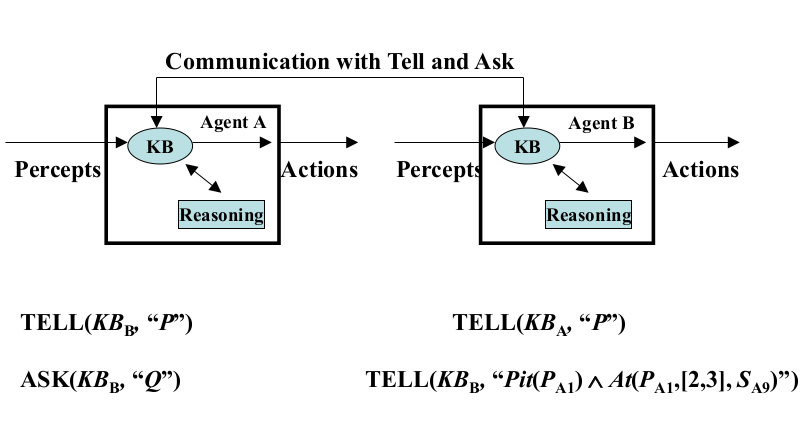
\includegraphics[scale=0.3]{img/tell and ask.png}
			\end{center}
			\item Kommunikation unter Verwendung von Formalen Sprachen: Agenten machen sich keine Annahmen über die interne Repräsentation der Sprache; Agenten teilen eine gemeinsame Sprache für die Kommunikation
			\begin{center}
				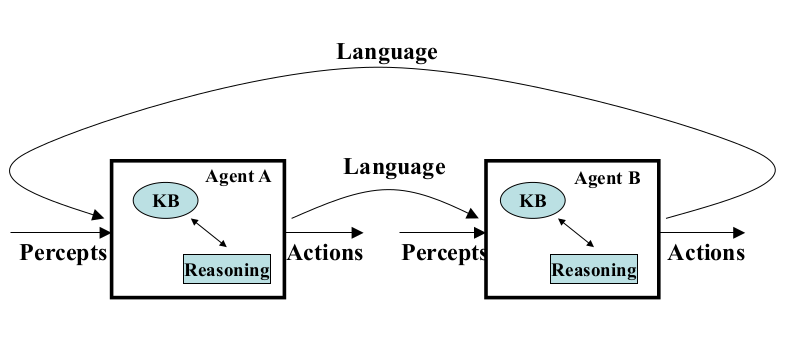
\includegraphics[scale=0.3]{img/formal language.png}
			\end{center}
		\end{itemize}
		\item Größtes Problem: Kommunikation ist zweideutig; Lösung durch Berücksichtigung des Contexts und der vorigen Kommunikationen
		\item Definition der Semantik auf Basis von Planung: bestimmte Prädikate welche in der jeweiligen precondition-delete-add Listen verwaltet werden
		\item Beispiel: request(s,h,$\phi$)
		\begin{itemize}
			\item pre: s glaubt h kann $\phi$ tun; s glaubt h glaubt h kann $\phi$; s glaubt s will $\phi$
			\item post: h glaubt s glaubt s will $\phi$
		\end{itemize}
	\end{itemize}
	\subsection{KQML und KIF}
	\begin{itemize}
		\item nun Betrachtung von Agent Communication Languages (ACLs) d.h. standard Formate für den Austausch von Nachrichten
		\item bekannteste ACL: KQML
		\item zwei Bestandteile: Wissens-Abfrage und -Manipulations Sprache (KQML) und Wissens-Austausch Format (KIF)
		\item KQML ist eine äußere Sprache welche verschiedene akzeptierbare Verben (performatives) definiert (Bsp: ask-if, perform, tell, reply)
		\item KIF ist eine Sprache für die Repräsentation des Nachrichteninhaltes (meistens sowas wie Common Lisp)
		\item für die Kommunikation müssen die Agenten das gleiche Verständnis von Ausdrücken haben (Was bedeutet Schalter1?), formale Definition in einer Ontology
	\end{itemize}
	\subsection{FIPA}
	\begin{itemize}
		\item neue Entwicklung der Agenten Standards inc. ACL
		\item Basisstrukltur ist ähnlich zu KQML: Permative + Housekeeping + Content
		\item INFORM und REQUEST sind die zwei Standard Permative in FIPA; der Rest wird auf Basis dieser definiert
		\item Bedeutung von INFORM und REQUEST hat zwei Parts: pre-condition (muss wahr sein damiot der Speech Act erfolgreich ist), rational effect (Ziel welches der Sender der Nachricht erreichen möchte)
		\item Beschreibung der pre-condtions usw als logischer Ausdruck
	\end{itemize}
	\subsection{Ontologien}
	\begin{itemize}
		\item Situation: Service Oriented Computing
		\item Alle Teilnehmer haben ein gemeinsames, gleiches Verständniss von Begriffen über eine Domäne (Ontologie) d.h. jeder Teilnehmer weiß genau was unter einem bestimmten Begriff zu verstehen ist
		\item Eine Ontologie beschreibt Begriffe und deren Relationen zu einander
		\item Ontologien unterstützen die Interaktion dadruch dass sie Begriffe eine Bedeutung geben
		\item Ontologien-Sprachen erlauben den User eine explizite und formale Konzeptionierung der Domäne
		\item Problem: je umfangreicher die Sprache desto schwieriger wird es daraus zu schließen
		\item Schließen in einer Ontology
		\begin{itemize}
			\item Klassenzugehörigkeit: Wenn x in der Klasse C und C eine Unterklasse von D, ist x auch in der Klasse D
			\item Klassenequivalenz: Wenn Klasse A ist equivalent zu B und B zu C denn ist A equivalent zu C
			\item Konsistenz: Wir haben X Instanzen von A und B aber  A und B sind disjunkt d.h. Fehler in der Ontologie
			\item Klassifikation: gegeben Eigenschaft-Werte-Paare für Klasse A, wenn x die Kriterien erfüllt ist x in A
		\end{itemize}
		\item Schließen ist wichtig für: Überprüfung der Ontologie und des Wissens; Überprüfung ob ungewollte Beziehungen der Klassen entstanden sind; automatische Zuordnung von Instanzen zu Klassen
		\item Überprüfungen sind wertvoll für: den Entwurf von großen Ontologien mit meheren Autoren; Integration und Verteilung anderer Ontologien an/von verschieden Quellen
	\end{itemize}
	\section{Wie sollten Agenten kommunizieren? Strategien und Protokolle}
	\subsection{Einführung}
	\begin{itemize}
		\item Kommunikation ist wichtig für die Verteilung von Aufgaben(Aufteilung von Teilaufgaben) und Ergebnissen (Teilergebnisse)
		\item Protokolle regeln die Interaktion zwischen Agenten
	\end{itemize}
	\subsection{Contract Net}
	\begin{itemize}
		\item Realisierung von Multi-Cast Kommunikation in Agenten-basierten Systemen
		\item zwei Rollen: Selector und Contractor
		\item Contract Net: Aufgabenverteilungs-Protokol für Aufgabenzuweisung
		\item Schritte:
		\begin{enumerate}
			\item Recognition: Feststellung des Problems
			\item Announcement: Mitteilung des Problems an alle Teilnehmer
			\item Bidding: Teilnehmer beantworten mit den erwarteten Kosten
			\item Awarding: Auftragsgeber belohnt den ausgewählten Teilnehmer
			\item Expediting: ???
		\end{enumerate}
		\item Recognition
		\begin{itemize}
			\item Agent nimmt Problem wahr
			\item Agent hat Ziel und: merkt dass er das Ziel nicht alleine erreichen kann (Nicht genügend Kapazität); merkt dass er dieses Ziel nicht alleine erreichen möchte (Deadline, Lösungsqualität)
		\end{itemize}
		\item Announcement
		\begin{itemize}
			\item Agent sendet Aufgabe incl. Spezifikation der Aufgabe an alle Teilnehmer
			\item Spezifikation beinhaltet: Aufgabenbeschreibung, Anforderungen (Deadlines, Qualität der Lösung), Meta-Informationen
			\item Announcement ist ein Broadcast
		\end{itemize}
		\item Bidding
		\begin{itemize}
			\item Agenten empfangen Announcement und entscheiden sich ob sie für die Aufgabe bieten möchten
			\item Faktoren: Agent muss entscheiden ob er in der Lage ist die Aufgabe zu bewältigen; Agent muss die Contraints ermitteln ggf. Preis
			\item wenn sie mitbieten wollen, senden Gebot (tender) an Aufgabensteller
		\end{itemize}
		\item Awarding \& Expediting
		\begin{itemize}
			\item Aufgabensteller muss aus den Geboten auswählen und entscheiden wer belohnt werden soll
			\item Ergebniss wird den teilnehmenden Agenten mitgeteilt
			\item Erfolgreicher Contractor (Teilnehmer) führt die Aufgabe aus
			\item ggf. Erweiterung der Contractor Beziehung um weitere unter Beziehungen: sub-contracting
		\end{itemize}
		\item Problem: Spezifikation von ...
		\begin{itemize}
			\item Aufgaben: gemeinsame Sprache der Agenten
			\item Lösungsqualität: Anforderungen (Ontologien), Werbungen und Reputation
			\item Auswahl von konkurierenden Angeboten: Prefärenzen
		\end{itemize}
	\end{itemize}
	\section{Verhandlungen}
	\subsection{Einführung}
	\begin{itemize}
		\item Wie können Agenten eine Übereinkunft treffen wenn sie sich egoistisch verhalten?
		\item Worst-Case: Null-Summen-Spiele d.h. keine Übereinkunft möglich ABER meistens die Möglichkeit ein kurzeitige Übereinkunft zu treffen zum allgmeinen Intersse
		\item Fähigkeiten der Verhandlung notwendig
		\item Verhandlungen werden durch einen Mechanismus (Protokoll) gesteuert
		\item Mechanismus = Regeln für das Treffen von Agenten
		\item Mechanismus-Design: Entwicklung von Mechanismen mit bestimmten Eigenschaften
		\item Mechanismus-Design Eigenschaften:
		\begin{itemize}
			\item Konvergenz und garantierter Erfolg
			\item Maximierung des Gemeinwohles
			\item Parto-Effizienz
			\item Individuelle Rationalität
			\item Stabilität
			\item Einfachheit
			\item Verteilung
		\end{itemize} 
	\end{itemize}
	\subsection{Verhandlung - Auktionen}
	\begin{itemize}
		\item Auktionen finden statt zwischen einen Auktionators und eine Menge von Bietern 
		\item Ziel: Auktionator möchte eine Zuweisung von Gütern (Ressourcen) an einen Bieter erreichen
		\item Meistens möchte Auktionator den maximalen Preis erreichen, die Bieter den minimalen
		\item Auktions-Parameter
		\begin{itemize}
			\item Güter haben: Privaten Wert, Allgemeinen Wert, Korrelierten Wert
			\item Gewinnerermittelung durch: erstes Gebot, zweites Gebot
			\item Gebote sind: für alle sichtbar (open cry); verborgen (sealed bid)
			\item Gebotsabgabe: einmalig (one shot), aufsteigend, absteigend
		\end{itemize}
	\end{itemize}
	\subsection{Englische Auktion}
	\begin{itemize}
		\item höchstes Gebot gewinnt, für alle sichtbar, aufsteigend
		\item Dominante Strategie: minimale Erhöhung des höchsten Gebotes bis Obergrenze erreicht, falls diese überschritten: Rückzug
		\item Anfällig: Fluch des Gewinners (Bezahlt meistens zuviel), Lockvögel (Agent arbeitet mit Auktionator zusammen und treibt den Preis künstlich in die Höhe)
	\end{itemize}
	\subsection{Holländische Auktion}
	\begin{itemize}
		\item offene Gebote, absteigend
		\item Auktionator startet mit hohen Startgebot
		\item Auktionator senkt Preis bis Agent ein Gebot zu dem Preis abgiebt
		\item Gewinner: Agent mit der Preisabgabe
	\end{itemize}
	\subsection{First-Price Sealed-Bid Auction}
	\begin{itemize}
		\item einmaliges Gebot, verborgen,
	\end{itemize}
	\section{???}
	\section{???}	
	\section{Blackboard}
	\subsection{Allgemein}
	\begin{itemize}
		\item indirekte Kommunikation d.h. keine direkte Kommunikation zwischen den Agenten sondern über ein Medium
		\item Kommunikation durch schreiben der Information auf Blackboard (zentraler Datenspeicher)
		\item Agenten können partielle Lösungen für das Problem dort veröffentlichen
		\item Zentrale Datenstruktur ist Flaschenhals ggf. muss irg welche Hierarchien verfügen
		\item subscripe-notify pattern: Agent bekündet Interesse über  bestimme Ereignisse, wenn Ereignis eintritt wird Agent benachrichtigt (proaktiv)
		\item Annahmen: verschiedene Agenten greifen asynchron auf die Datenstruktur zu; ????
		\item Wissensquelle: Agent drückt ein Teil der Lösung aus; ???
		\item (??? IRG WAS MIT PRECONDITIONS ???)
		\item Verschiedene Hierarchien für Tests (??? PRECONDITIONS ???)
		\item Modularität: Man kann einzelne WQ des System entwickeln ohne zu wissen welche anderen WQ es gibt (also indirekte Kommunikation)
		\item Interessant: Wie verändert sich die Systemleistung durch Austausch einzelner WQ?
		\item Kommunikation:
		\begin{enumerate}
			\item Sammlung von Daten über Events für zukünftige Anwendung
			\item Detektion von Event welche vorige Annahme widersprechen (???)
		\end{enumerate}
		\item Lokale Kontexte: Jeder hat eigene lokalen Abbild der Datenbank der von Interesse ist, Übertragung neuer Events an entsprechende Interessierte
		\item (??? Folie über sprungen zu Integrität ???)
		\item jeder Agent hat eigene Datenbank, Verteilung der Information über Blackboard; lokale Datenbanken bilden zusammen globale Datenbanken
	\end{itemize}
	\subsection{Alternative Architekturen}
	\begin{itemize}
		\item Beispiel: Speech Understanding,
		\item Ansatz 1: Pipe-and-Filter Architektur; Problem: keine klare Trennung, ggf Wissen aus unterschiedlichen Quellen notwendig d.h. Architektur wird unnötige komplex
		\item Ansatz 2: Object-Orientierte-Architektur; Problem: nicht flexibel da jede WQ wissen muss was eine andere WQ produzieren kann; Lösung: Client-Broker Ansatz aber recht komplex
		\item Ansatz 3: Sichten-System; Problem: 
		\item Besser: Alle Prozesse kommunizieren über Blackboard, Ziel: Wissensverteilung der Partiellen Lösungen
	\end{itemize}

\end{document}